\documentclass[11pt,a4paper]{article}

\usepackage[T1]{fontenc}
\usepackage[utf8]{inputenc}
\usepackage[margin=2.4cm]{geometry}
\usepackage{amsmath,amssymb}
\usepackage{booktabs}
\usepackage{array}
\usepackage{tikz}
\usepackage{xcolor}
\usepackage[most]{tcolorbox}
\usepackage{enumitem}
\usepackage{listings}
\usepackage{hyperref}

% ---- style code Python ----
\definecolor{codebg}{HTML}{F6F8FA}
\definecolor{codekw}{HTML}{A626A4}
\definecolor{codestr}{HTML}{50A14F}
\definecolor{codecom}{HTML}{A0A1A7}
\definecolor{codenum}{HTML}{986801}
\lstdefinestyle{py}{
  language=Python, backgroundcolor=\color{codebg}, basicstyle=\ttfamily\small,
  keywordstyle=\color{codekw}\bfseries, stringstyle=\color{codestr},
  commentstyle=\color{codecom}\itshape, numberstyle=\tiny\color{codecom},
  numbers=left, numbersep=7pt, showstringspaces=false, breaklines=true,
  frame=single, rulecolor=\color{codecom!40}, framesep=5pt,
  keywordstyle=[2]\color{codenum}, morekeywords=[2]{}, columns=fullflexible,
  literate={é}{{\'e}}1 {è}{{\`e}}1 {à}{{\`a}}1 {ê}{{\^e}}1 {î}{{\^i}}1 {ô}{{\^o}}1 {ç}{{\c c}}1
}

\usetikzlibrary{arrows.meta,positioning,calc}
\hypersetup{colorlinks=true,linkcolor=blue!55!black,urlcolor=blue!55!black}

\definecolor{coreblue}{HTML}{1F5C99}
\definecolor{coregrey}{HTML}{4A4A4A}

% ---- boîtes ----
\newtcolorbox{defbox}[1]{colback=coreblue!5,colframe=coreblue,
  fonttitle=\bfseries,title={#1},boxrule=0.6pt,left=6pt,right=6pt,top=4pt,bottom=4pt}
\newtcolorbox{rembox}[1]{colback=orange!6,colframe=orange!70!black,
  fonttitle=\bfseries,title={#1},boxrule=0.6pt,left=6pt,right=6pt,top=4pt,bottom=4pt}

\newcommand{\NP}{\mathrm{NP}}
\newcommand{\PTDF}{\mathrm{PTDF}}
\newcommand{\RAM}{\mathrm{RAM}}
\newcommand{\Fmax}{F^{\max}}
\newcommand{\Fref}{F^{\mathrm{ref}}}
\newcommand{\FRM}{\mathrm{FRM}}
\newcommand{\GSK}{\mathrm{GSK}}

\title{\vspace{-1.2cm}\textbf{Le calcul \textit{Flow-Based}}\\[2pt]
\large PTDF, RAM, CNEC et sommets du domaine\\[6pt]
\normalsize\textit{avec un exemple complet à trois zones}}
\author{}
\date{}

\renewcommand{\contentsname}{Table des matières}

\begin{document}
\maketitle
\vspace{-1.4cm}
\hrule
\vspace{0.4cm}

\tableofcontents
\vspace{0.6cm}
\hrule

% =====================================================================
\section{Principe général du couplage flow-based}

Le couplage de marché \emph{flow-based} (FB) est la méthode d'allocation
de capacité transfrontalière utilisée en Europe (région \emph{Core},
Nordic, etc.). Contrairement à l'approche NTC (\emph{Net Transfer
Capacity}), qui fixe \emph{a priori} des capacités d'échange rigides entre
paires de zones, le flow-based ne fixe pas de limites bilatérales : il
calcule un \textbf{domaine} de positions nettes admissibles à partir de la
manière dont les échanges commerciaux chargent \emph{physiquement} le
réseau.

\begin{defbox}{Position nette d'une zone}
La position nette $\NP_z$ d'une zone $z$ est le solde
export\,$-$\,import de cette zone : positive si la zone exporte, négative
si elle importe. Sur le périmètre couplé, les positions nettes se
compensent :
\[
  \sum_{z} \NP_z = 0 .
\]
Avec $N$ zones, le domaine vit donc dans un espace de dimension $N-1$.
\end{defbox}

La chaîne de calcul se résume en trois briques, qui s'enchaînent
logiquement :
\begin{enumerate}[nosep]
  \item les \textbf{PTDF} donnent les \emph{coefficients} des contraintes
        (comment un échange charge chaque élément de réseau) ;
  \item le \textbf{RAM} donne le \emph{second membre} des contraintes
        (la marge restante sur chaque élément) ;
  \item chaque \textbf{CNEC} produit une contrainte linéaire ; leur
        intersection forme un \textbf{polytope} convexe dont on extrait
        les \textbf{sommets} (\textit{vertices}) et dont la
        \textbf{projection 2D} donne la vue lisible du domaine.
\end{enumerate}

% =====================================================================
\section{Les PTDF : les coefficients des contraintes}

Le \emph{Power Transfer Distribution Factor} mesure la \textbf{sensibilité}
du flux physique sur un élément de réseau à une variation d'injection :
« si j'injecte 1~MW ici et que je le soutire au n\oe{}ud de référence
(\emph{slack}), quelle fraction transite par cette branche ? ». Il découle
de la topologie et des réactances du réseau (calcul de type
\emph{load-flow} continu, dit DC).

\paragraph{PTDF nodal.} Sensibilité du flux sur une branche $c$ à une
injection au n\oe{}ud $n$, mesurée relativement au n\oe{}ud de référence.
C'est la grandeur brute issue du modèle de réseau commun.

\paragraph{PTDF zonal.} C'est celui qui entre dans le flow-based. On agrège
les PTDF nodaux d'une zone au moyen d'une clé de répartition de la
production, la \textbf{GSK} (\emph{Generation Shift Key}), qui répartit la
variation de position nette d'une zone sur ses n\oe{}uds :
\[
  \PTDF^{\text{zonal}}_{c,z}
   \;=\; \sum_{n \in z} \GSK_{n,z}\;\PTDF^{\text{nodal}}_{c,n},
   \qquad \sum_{n\in z}\GSK_{n,z}=1 .
\]
Le PTDF zonal $\PTDF_{c,z}$ indique de combien varie le flux sur le CNEC
$c$ lorsque la zone $z$ augmente son export net de 1~MW. \textbf{Ce sont
exactement les coefficients} des contraintes linéaires du domaine.

\begin{rembox}{Rappel : d'où viennent les PTDF (load-flow DC)}
Dans un réseau maillé, un transfert se répartit sur les chemins parallèles
\emph{inversement} à leur réactance. Pour un triangle de trois lignes de
réactances égales, un transfert de A vers C se répartit ainsi :
$2/3$ sur la liaison directe A--C, et $1/3$ sur le chemin A--B--C. Ce sont
ces fractions qui constitueront les PTDF de notre exemple.
\end{rembox}

\subsection{Formulation matricielle (load-flow DC)}
\label{sec:matrice}

Le PTDF se dérive du load-flow \textbf{linéarisé} (DC), sous trois
hypothèses : modules de tension $\approx 1$~p.u., résistances négligées
devant les réactances ($r \ll x$), et angles faibles
($\sin\theta \approx \theta$). Le flux actif sur une branche $k$ reliant
les n\oe{}uds $i$ et $j$ devient \emph{linéaire} :
\[
  F_k \;=\; \frac{\theta_i - \theta_j}{x_k}
       \;=\; b_k\,(\theta_i - \theta_j),
       \qquad b_k = 1/x_k .
\]

On introduit trois matrices ($n$ n\oe{}uds, $m$ branches) :
\begin{itemize}[nosep,leftmargin=1.4em]
  \item $A$ : matrice d'\textbf{incidence} branche$\times$n\oe{}ud
        ($m\times n$), avec $+1$ à l'origine et $-1$ à l'extrémité de
        chaque branche ;
  \item $B_d = \mathrm{diag}(b_k)$ : susceptances de branche
        ($m\times m$) ;
  \item $B_{\mathrm{bus}} = A^{\top} B_d\, A$ : matrice nodale
        (\emph{Laplacien} pondéré du réseau, $n\times n$).
\end{itemize}

Les injections nodales $P$ et les angles $\theta$ sont alors reliés par
$P = B_{\mathrm{bus}}\,\theta$. La matrice $B_{\mathrm{bus}}$ est
\textbf{singulière} (rang $n-1$) : les angles ne sont définis qu'à une
constante additive près. On lève l'indétermination en choisissant un
\textbf{n\oe{}ud de référence} (\emph{slack}) : on retire sa ligne et sa
colonne, on inverse la sous-matrice, puis on ré-emboîte le résultat dans
une matrice $X$ ($n\times n$) dont la ligne et la colonne du slack sont
nulles. On a alors $\theta = X P$, d'où les flux :
\[
  F \;=\; B_d\, A\, \theta \;=\; \underbrace{B_d\, A\, X}_{\displaystyle \mathrm{PTDF}}\; P .
\]

\begin{defbox}{Matrice PTDF}
\[
  \boxed{\;\mathrm{PTDF} \;=\; B_d\, A\, X\;}\qquad (m\times n)
\]
$\mathrm{PTDF}_{k,i} = \partial F_k/\partial P_i$ est la variation de flux
sur la branche $k$ pour 1~MW injecté au n\oe{}ud $i$ et \emph{soutiré au
slack}. Par construction $\mathrm{PTDF}_{k,\text{slack}} = 0$. Le PTDF ne
dépend que des réactances \emph{relatives} et de la topologie, jamais du
point de fonctionnement (conséquence de la linéarité du DC).
\end{defbox}

\subsection{Du nodal au zonal : la GSK}
\label{sec:gsk}

La matrice $\mathrm{PTDF}$ ci-dessus est \emph{nodale}. Le flow-based
raisonne par \emph{zone} : on regroupe les n\oe{}uds d'une zone au moyen
d'une matrice de clés de répartition $\mathrm{GSK}$ ($n\times Z$, dont
chaque colonne somme à 1). Le passage nodal~$\to$~zonal est alors un simple
produit matriciel :
\[
  \boxed{\;\mathrm{PTDF}^{\text{zonal}} \;=\; \mathrm{PTDF}^{\text{nodal}}\cdot \mathrm{GSK}\;}\qquad (m\times Z).
\]
Chaque colonne du résultat est la \emph{moyenne pondérée par la GSK} des
colonnes nodales de la zone. Deux variantes usuelles :
\begin{itemize}[nosep,leftmargin=1.4em]
  \item \textbf{zone-à-hub} : PTDF mesuré par rapport au slack/hub
        (ce que l'on vient d'écrire) ;
  \item \textbf{zone-à-zone} : $\mathrm{PTDF}_A - \mathrm{PTDF}_B$,
        sensibilité à un échange bilatéral $A\!\to\!B$.
\end{itemize}

\begin{rembox}{Effet d'une contingence sur le PTDF}
Après la perte d'une branche $\ell$, la topologie change, donc les PTDF
aussi. On peut recalculer $X$ sur le réseau amputé, ou utiliser les
\textbf{LODF} (\emph{Line Outage Distribution Factors}) :
\[
  \mathrm{PTDF}^{(\ell)}_{k,i} \;=\; \mathrm{PTDF}_{k,i}
     \;+\; \mathrm{LODF}_{k,\ell}\,\mathrm{PTDF}_{\ell,i}.
\]
Ce sont ces PTDF post-incident qui alimentent les contraintes de CNEC.
\end{rembox}

% =====================================================================
\section{Le RAM : le second membre des contraintes}

Le \emph{Remaining Available Margin} est la marge encore disponible sur un
CNEC pour absorber les échanges commerciaux :
\[
  \boxed{\;\RAM_c \;=\; \Fmax_c \;-\; \Fref_c \;-\; \FRM_c\;}
\]
\begin{itemize}[nosep,leftmargin=1.4em]
  \item $\Fmax_c$ : flux physique maximal admissible (limite thermique,
        éventuellement saisonnière) ;
  \item $\Fref_c$ ($F_0$) : \emph{flux de référence} déjà présent dans le
        modèle de réseau pour le programme de référence — la part de
        capacité déjà consommée avant le couplage ;
  \item $\FRM_c$ : \emph{Flow Reliability Margin}, marge de fiabilité
        couvrant les incertitudes entre le calcul \emph{day-ahead} et le
        temps réel (déterminée statistiquement).
\end{itemize}

\begin{rembox}{Règle du \textit{minRAM} (70 \%)}
Le règlement européen 2019/943 (\emph{Clean Energy Package}, art.~16) impose
qu'au moins \textbf{70~\%} de la capacité de chaque élément soit offerte aux
échanges transfrontaliers :
\[
  \RAM_c \;\ge\; 0{,}7 \times \Fmax_c .
\]
Si le RAM calculé tombe en dessous, un ajustement le relève à ce plancher.
\end{rembox}

% =====================================================================
\section{Le CNEC : la brique qui définit les contraintes}

\begin{defbox}{CNEC = CNE + Contingency}
Un \textbf{CNEC} (\emph{Critical Network Element and Contingency}) associe :
\begin{itemize}[nosep,leftmargin=1.4em]
  \item un \textbf{CNE} (\emph{Critical Network Element}) : ligne,
        transformateur ou interconnexion fortement impacté par les échanges
        et susceptible d'être congestionné ;
  \item une \textbf{contingency} : un scénario de défaillance, typiquement
        en $N\!-\!1$ (perte d'un élément du réseau).
\end{itemize}
Un CNEC représente donc « cet élément surveillé, dans la situation où tel
autre élément est hors service ».
\end{defbox}

Le flux sur le CNEC $c$ s'écrit, en fonction des positions nettes :
\[
  F_c \;=\; \Fref_c \;+\; \sum_z \PTDF_{c,z}\,\bigl(\NP_z - \NP_z^{\mathrm{ref}}\bigr).
\]
La condition de non-congestion $F_c \le \Fmax_c$ devient, en posant
$\Delta\NP_z = \NP_z - \NP_z^{\mathrm{ref}}$ :
\[
  \boxed{\;\sum_z \PTDF_{c,z}\,\Delta\NP_z \;\le\; \RAM_c\;}
\]
\textbf{Chaque CNEC $=$ une inégalité linéaire $=$ une face du domaine.}
La branche pouvant être chargée dans les deux sens, on écrit en pratique
une contrainte $+\Fmax$ et une contrainte $-\Fmax$ par CNEC.

% =====================================================================
\section{Le domaine flow-based et ses sommets}

L'ensemble de toutes les contraintes de CNEC définit un \textbf{polytope
convexe} dans l'espace des positions nettes : c'est le \emph{domaine
flow-based}, l'ensemble de toutes les combinaisons de $\NP_z$ respectant
simultanément \emph{toutes} les contraintes du réseau.

\begin{defbox}{Sommets (\textit{vertices})}
Les \textbf{sommets} sont les points extrêmes — les « coins » — du polytope,
c.-à-d.\ les intersections des hyperplans des contraintes actives. Ils
servent à décrire, vérifier et visualiser le domaine, et caractérisent les
échanges maximaux réalisables.
\end{defbox}

\paragraph{Projection 2D.} Le domaine ayant $N-1$ dimensions (plusieurs
dizaines pour Core), on le \textbf{projette} sur deux axes en fixant les
autres positions nettes. Chaque contrainte devient alors une \emph{droite},
la région admissible un \textbf{polygone convexe} : ses \emph{côtés} sont
les CNEC contraignants, ses \emph{sommets} les intersections de ces droites.

% =====================================================================
\section{Exemple complet à trois zones}

\subsection{Réseau et hypothèses}

On considère trois zones A, B, C, chacune réduite à un n\oe{}ud (la GSK est
donc triviale, $\GSK=1$), reliées en triangle par trois lignes de
réactances \emph{égales} :
\[
  L_{AB}\ (A\!\to\!B),\qquad L_{BC}\ (B\!\to\!C),\qquad L_{AC}\ (A\!\to\!C).
\]

\begin{center}
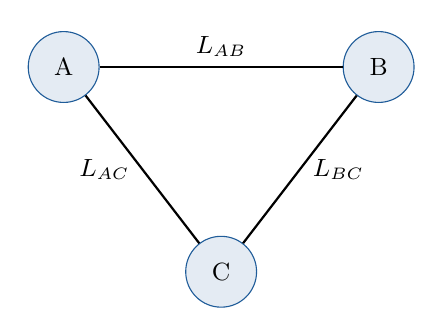
\begin{tikzpicture}[scale=1.0,every node/.style={font=\small}]
  \node[circle,draw=coreblue,fill=coreblue!12,minimum size=9mm] (A) at (0,0) {A};
  \node[circle,draw=coreblue,fill=coreblue!12,minimum size=9mm] (B) at (4,0) {B};
  \node[circle,draw=coreblue,fill=coreblue!12,minimum size=9mm] (C) at (2,-2.6) {C};
  \draw[thick] (A)--(B) node[midway,above]{$L_{AB}$};
  \draw[thick] (B)--(C) node[midway,right=1pt]{$L_{BC}$};
  \draw[thick] (A)--(C) node[midway,left=1pt]{$L_{AC}$};
\end{tikzpicture}
\end{center}

On choisit \textbf{C comme n\oe{}ud de référence} (\emph{slack}) et un
programme de référence \emph{à plat} ($\NP^{\mathrm{ref}}=0$, donc
$\Fref=0$ sur toutes les lignes). Les variables du domaine sont alors
$\Delta\NP_A$ et $\Delta\NP_B$, avec
$\Delta\NP_C = -(\Delta\NP_A + \Delta\NP_B)$.

\subsection{Calcul des PTDF}

Un transfert d'une zone vers le slack C se répartit inversement aux
réactances (cf.\ encadré \S2). On obtient, pour chaque ligne, les PTDF
zonaux vis-à-vis de A et de B ; comme C est le slack, $\PTDF_{\bullet,C}=0$.

\begin{itemize}[nosep,leftmargin=1.4em]
  \item \textbf{Injection en A} (soutirage en C) : $2/3$ sur $L_{AC}$,
        $1/3$ sur $L_{AB}$ puis sur $L_{BC}$.
  \item \textbf{Injection en B} (soutirage en C) : $2/3$ sur $L_{BC}$
        (direct), $1/3$ par le chemin B$\to$A$\to$C, soit $-1/3$ sur
        $L_{AB}$ (sens B$\to$A) et $+1/3$ sur $L_{AC}$.
\end{itemize}

On ajoute un \textbf{CNEC avec contingence} : la ligne $L_{BC}$ surveillée
\emph{après déclenchement de $L_{AC}$}. Le réseau devient radial
(A--B--C) : tout transfert depuis A ou B vers C passe alors intégralement
par $L_{BC}$, d'où $\PTDF_A = \PTDF_B = 1$.

\subsection{Vérification par la matrice \texorpdfstring{$B$}{B}}

Reprenons la formulation matricielle du \S\ref{sec:matrice} sur ce réseau
(n\oe{}uds ordonnés $A,B,C$ ; lignes $L_{AB},L_{BC},L_{AC}$ ; $b_k=1$). La
matrice d'incidence et le Laplacien valent :
\[
  A = \begin{pmatrix} 1 & -1 & 0\\ 0 & 1 & -1\\ 1 & 0 & -1\end{pmatrix},
  \qquad
  B_{\mathrm{bus}} = A^{\top}A =
  \begin{pmatrix} 2 & -1 & -1\\ -1 & 2 & -1\\ -1 & -1 & 2\end{pmatrix}.
\]
On retire la ligne/colonne du slack $C$, on inverse le bloc $2\times2$
restant, puis on ré-emboîte (ligne/colonne $C$ nulle) :
\[
  \begin{pmatrix} 2 & -1\\ -1 & 2\end{pmatrix}^{-1}
   = \tfrac13\begin{pmatrix} 2 & 1\\ 1 & 2\end{pmatrix}
  \;\Longrightarrow\;
  X = \tfrac13\begin{pmatrix} 2 & 1 & 0\\ 1 & 2 & 0\\ 0 & 0 & 0\end{pmatrix}.
\]
Enfin $\mathrm{PTDF} = B_d\,A\,X = A\,X$ (car $B_d=I$ ici) :
\[
  \mathrm{PTDF} =
  \begin{array}{r|ccc}
     & A & B & C\\\hline
    L_{AB} & +\tfrac13 & -\tfrac13 & 0\\
    L_{BC} & +\tfrac13 & +\tfrac23 & 0\\
    L_{AC} & +\tfrac23 & +\tfrac13 & 0
  \end{array}
\]
On retrouve exactement les valeurs du tableau des CNEC ci-dessous. Ces
mêmes valeurs seront reproduites numériquement par pypowsybl au
\S\ref{sec:pypowsybl}.

\subsection{Table des CNEC}

Limites thermiques $\Fmax$ et marges $\FRM$ choisies ci-dessous ; la
référence étant à plat, $\Fref=0$ et $\RAM = \Fmax - \FRM$ (identique dans
les deux sens de la ligne).

\begin{center}
\renewcommand{\arraystretch}{1.25}
\begin{tabular}{c l c c c c c c}
\toprule
\# & CNE & Contingence & $\PTDF_A$ & $\PTDF_B$ & $\Fmax$ & $\FRM$ & $\RAM$ \\
\midrule
1 & $L_{AB}$ & --- ($N$)      & $+\tfrac13$ & $-\tfrac13$ & 250 & 50  & \textbf{200} \\
2 & $L_{BC}$ & --- ($N$)      & $+\tfrac13$ & $+\tfrac23$ & 360 & 60  & \textbf{300} \\
3 & $L_{AC}$ & --- ($N$)      & $+\tfrac23$ & $+\tfrac13$ & 360 & 60  & \textbf{300} \\
4 & $L_{BC}$ & $L_{AC}$ H.S.  & $+1$        & $+1$        & 600 & 100 & \textbf{500} \\
\bottomrule
\end{tabular}
\end{center}

\begin{rembox}{Pourquoi $\Fmax$ diffère pour $L_{BC}$ entre les CNEC 2 et 4 ?}
Le CNEC~2 utilise la limite \emph{permanente} de $L_{BC}$ (360~MW), tandis
que le CNEC~4 est un état \emph{post-incident} : les gestionnaires de réseau
admettent alors une limite \emph{d'urgence de courte durée} plus élevée
(600~MW). C'est une pratique courante et réaliste. On vérifie par ailleurs
le \emph{minRAM} : $0{,}7\times\Fmax$ vaut $175,\,252,\,252,\,420$~MW pour
les CNEC 1 à 4 ; tous les RAM retenus lui sont supérieurs, aucun ajustement
n'est nécessaire.
\end{rembox}

\subsection{Les inéquations du domaine}

En posant $x=\Delta\NP_A$ et $y=\Delta\NP_B$ (en MW), chaque CNEC donne deux
contraintes ($\pm$). En multipliant par 3 pour éliminer les fractions :

\begin{center}
\renewcommand{\arraystretch}{1.3}
\begin{tabular}{c l l}
\toprule
CNEC & Contrainte « + » & Contrainte « $-$ » \\
\midrule
1 ($L_{AB}$)          & $x - y \le 600$   & $x - y \ge -600$ \\
2 ($L_{BC}$)          & $x + 2y \le 900$  & $x + 2y \ge -900$ \\
3 ($L_{AC}$)          & $2x + y \le 900$  & $2x + y \ge -900$ \\
4 ($L_{BC}\,|\,L_{AC}$) & $x + y \le 500$ & $x + y \ge -500$ \\
\bottomrule
\end{tabular}
\end{center}

L'intersection de ces huit demi-plans est un \textbf{octogone} : les huit
contraintes sont toutes actives (chacune porte un côté du domaine).

\subsection{Le domaine projeté et ses sommets}

\begin{center}
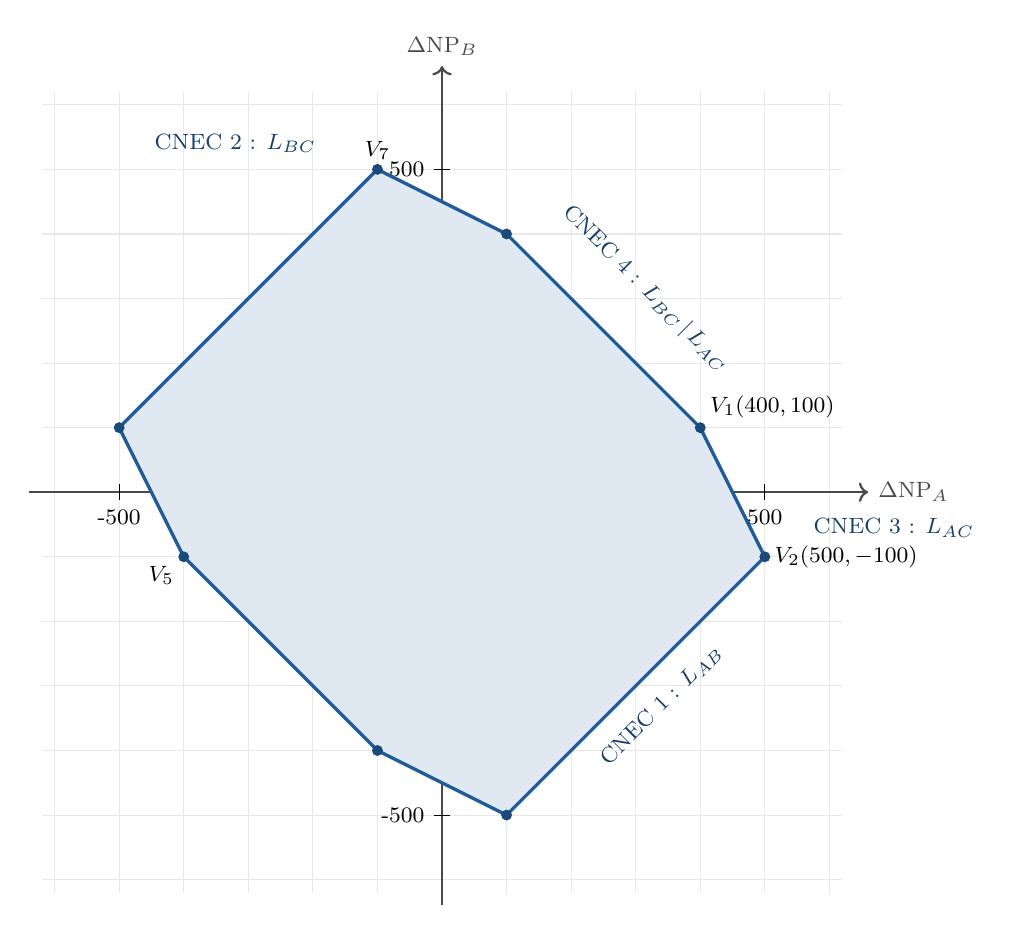
\begin{tikzpicture}[scale=0.82,every node/.style={font=\footnotesize}]
  % grille
  \foreach \i in {-6,...,6} {\draw[gray!18] (\i,-6.2)--(\i,6.2);}
  \foreach \i in {-6,...,6} {\draw[gray!18] (-6.2,\i)--(6.2,\i);}
  % axes
  \draw[->,coregrey,thick] (-6.4,0)--(6.6,0) node[right]{$\Delta\NP_A$};
  \draw[->,coregrey,thick] (0,-6.4)--(0,6.6) node[above]{$\Delta\NP_B$};
  \foreach \i/\lbl in {-5/-500,5/500}
     {\draw (\i,0.12)--(\i,-0.12) node[below]{\lbl};
      \draw (0.12,\i)--(-0.12,\i) node[left]{\lbl};}
  % domaine (octogone), échelle 1 unité = 100 MW
  \filldraw[fill=coreblue!14,draw=coreblue,very thick]
    (5,-1)--(4,1)--(1,4)--(-1,5)--(-5,1)--(-4,-1)--(-1,-4)--(1,-5)--cycle;
  % sommets
  \foreach \p in {(5,-1),(4,1),(1,4),(-1,5),(-5,1),(-4,-1),(-1,-4),(1,-5)}
     \fill[coreblue!80!black] \p circle (2.4pt);
  % étiquettes de sommets clés
  \node[above right] at (4,1) {$V_1(400,100)$};
  \node[right] at (5,-1) {$V_2(500,-100)$};
  \node[above] at (-1,5) {$V_7$};
  \node[below left] at (-4,-1) {$V_5$};
  % étiquettes d'arêtes = CNEC
  \node[coreblue!70!black,rotate=-45] at (3.15,3.15) {CNEC 4 : $L_{BC}\,|\,L_{AC}$};
  \node[coreblue!70!black] at (7.0,-0.55) {CNEC 3 : $L_{AC}$};
  \node[coreblue!70!black] at (-3.2,5.4) {CNEC 2 : $L_{BC}$};
  \node[coreblue!70!black,rotate=45] at (3.4,-3.3) {CNEC 1 : $L_{AB}$};
\end{tikzpicture}
\end{center}

\noindent Les huit sommets de l'octogone (avec
$\Delta\NP_C = -(x+y)$) :

\begin{center}
\renewcommand{\arraystretch}{1.2}
\begin{tabular}{c c c c l}
\toprule
Sommet & $\Delta\NP_A$ & $\Delta\NP_B$ & $\Delta\NP_C$ & CNEC actifs \\
\midrule
$V_1$ & $400$  & $100$  & $-500$ & 3 \& 4 \\
$V_2$ & $500$  & $-100$ & $-400$ & 1 \& 3 \\
$V_3$ & $100$  & $-500$ & $+400$ & 1 \& 2 \\
$V_4$ & $-100$ & $-400$ & $+500$ & 2 \& 4 \\
$V_5$ & $-400$ & $-100$ & $+500$ & 3 \& 4 \\
$V_6$ & $-500$ & $100$  & $+400$ & 1 \& 3 \\
$V_7$ & $-100$ & $500$  & $-400$ & 1 \& 2 \\
$V_8$ & $100$  & $400$  & $-500$ & 2 \& 4 \\
\bottomrule
\end{tabular}
\end{center}

\paragraph{Lecture.} Au sommet $V_1$, A et B exportent
($+400$ et $+100$~MW) et C importe $500$~MW ; les contraintes actives sont
le CNEC~3 ($L_{AC}$) et le CNEC~4 ($L_{BC}$ post-incident) — cohérent, car
un fort export vers C sature les lignes reliées à~C. C'est précisément la
direction où le réseau limite le marché.

\begin{rembox}{Effet d'un flux de référence $\Fref \neq 0$}
Si l'on avait par exemple $\Fref = 90$~MW sur $L_{BC}$, la contrainte « + »
du CNEC~2 deviendrait $\RAM = 360-90-60 = 210$~MW, soit
$x + 2y \le 630$, tandis que le sens « $-$ » gagnerait de la marge :
$x + 2y \ge -(360+90-60) = -390$. Le domaine se retrouverait
\emph{décalé et asymétrique} : c'est l'effet réel des flux de bouclage
(\emph{loop flows}) et de la situation de référence sur la forme du domaine.
\end{rembox}

% =====================================================================
\section{Mise en \oe{}uvre avec \texttt{pypowsybl}}
\label{sec:pypowsybl}

On reconstruit le triangle dans \texttt{pypowsybl} (moteur
\emph{OpenLoadFlow}) et l'on calcule les PTDF par analyse de sensibilité DC.
L'objectif est de montrer concrètement le \textbf{passage du nodal au
zonal}.

\subsection{Construction du réseau et slack}

Trois n\oe{}uds, trois lignes de réactance identique, une injection
(générateur) par n\oe{}ud. Le point clé est de forcer un \textbf{slack
unique} sur le n\oe{}ud C, via l'identifiant de son \emph{voltage level} :

\begin{lstlisting}[style=py]
import pypowsybl as pp

n = pp.network.create_empty("triangle-3-zones")
n.create_substations(id=["S_A", "S_B", "S_C"])
n.create_voltage_levels(id=["VL_A", "VL_B", "VL_C"],
    substation_id=["S_A", "S_B", "S_C"],
    topology_kind=["BUS_BREAKER"]*3, nominal_v=[400.0]*3)
n.create_buses(id=["A", "B", "C"],
    voltage_level_id=["VL_A", "VL_B", "VL_C"])

X = 10.0                                   # meme reactance sur les 3 lignes
n.create_lines(id=["L_AB", "L_BC", "L_AC"],
    voltage_level1_id=["VL_A", "VL_B", "VL_A"], bus1_id=["A", "B", "A"],
    voltage_level2_id=["VL_B", "VL_C", "VL_C"], bus2_id=["B", "C", "C"],
    r=[0.0]*3, x=[X, X, X],
    g1=[0.0]*3, b1=[0.0]*3, g2=[0.0]*3, b2=[0.0]*3)

n.create_generators(id=["G_A", "G_B", "G_C"],       # 1 injection / noeud
    voltage_level_id=["VL_A", "VL_B", "VL_C"], bus_id=["A", "B", "C"],
    target_p=[100.0, 100.0, 0.0], min_p=[-1e3]*3, max_p=[1e3]*3,
    target_q=[0.0]*3, voltage_regulator_on=[False]*3)
n.create_loads(id=["LD_C"], voltage_level_id=["VL_C"], bus_id=["C"],
    p0=[200.0], q0=[0.0])

# Mode DC + slack UNIQUE force sur le noeud C (via son voltage level)
lf = pp.loadflow.Parameters(dc=True, distributed_slack=False,
    provider_parameters={"slackBusSelectionMode": "NAME",
                         "slackBusesIds": "VL_C"})
params = pp.sensitivity.Parameters(load_flow_parameters=lf)
branches = ["L_AB", "L_BC", "L_AC"]
\end{lstlisting}

\subsection{PTDF nodal : variables = injections}

Pour le PTDF \emph{nodal}, les variables de sensibilité sont les
\textbf{injections} (les générateurs, un par n\oe{}ud) :

\begin{lstlisting}[style=py]
sa = pp.sensitivity.create_dc_analysis()
sa.add_branch_flow_factor_matrix(branches_ids=branches,
                                 variables_ids=["G_A", "G_B", "G_C"])
res = sa.run(n, params, provider="OpenLoadFlow")
print(res.get_sensitivity_matrix())      # PTDF nodal
print(res.get_reference_matrix())         # flux de reference
\end{lstlisting}

\noindent Résultat (lignes = injections, colonnes = branches) :
\begin{center}\ttfamily\small
\begin{tabular}{lrrr}
\toprule
 & L\_AB & L\_BC & L\_AC \\
\midrule
G\_A & $+0.3333$ & $+0.3333$ & $+0.6667$ \\
G\_B & $-0.3333$ & $+0.6667$ & $+0.3333$ \\
G\_C & $+0.0000$ & $+0.0000$ & $+0.0000$ \\
\bottomrule
\end{tabular}
\end{center}
\noindent Identique à la matrice $B_d A X$ calculée à la main, et
$\PTDF_{\bullet,C}=0$ (C est le slack). Les flux de référence retournés sont
$L_{AB}=0$, $L_{BC}=100$, $L_{AC}=100$~MW.

\subsection{Passage au zonal : la GSK}

\textbf{C'est l'étape centrale.} On ne change pas de réseau : on regroupe
les injections en \textbf{zones} au moyen de clés de répartition
(\emph{shift keys}), puis on déclare ces zones comme variables. Trois
appels suffisent :

\begin{lstlisting}[style=py]
# 1) definir les zones a partir des injections + GSK (shift keys)
zA = pp.sensitivity.create_zone_from_injections_and_shift_keys("A", ["G_A"], [1.0])
zB = pp.sensitivity.create_zone_from_injections_and_shift_keys("B", ["G_B"], [1.0])
zC = pp.sensitivity.create_zone_from_injections_and_shift_keys("C", ["G_C"], [1.0])

sa2 = pp.sensitivity.create_dc_analysis()
sa2.set_zones([zA, zB, zC])                       # 2) attacher les zones
sa2.add_branch_flow_factor_matrix(branches_ids=branches,
                                  variables_ids=["A", "B", "C"])  # 3) variables = ZONES
res2 = sa2.run(n, params, provider="OpenLoadFlow")
print(res2.get_sensitivity_matrix())              # PTDF zonal (zone -> hub)
\end{lstlisting}

\begin{defbox}{La seule différence nodal $\to$ zonal, côté code}
\begin{itemize}[nosep,leftmargin=1.4em]
  \item \textbf{Nodal} : \texttt{variables\_ids = ["G\_A","G\_B","G\_C"]}
        (des \emph{injections}).
  \item \textbf{Zonal} : on crée les zones avec
        \texttt{create\_zone\_from\_injections\_and\_shift\_keys}, on les
        attache avec \texttt{set\_zones(...)}, et
        \texttt{variables\_ids = ["A","B","C"]} (des \emph{zones}).
\end{itemize}
En interne, pypowsybl applique exactement
$\mathrm{PTDF}^{\text{zonal}} = \mathrm{PTDF}^{\text{nodal}}\cdot\mathrm{GSK}$.
\end{defbox}

Ici chaque zone ne contient qu'un n\oe{}ud, donc la GSK est la matrice
identité et le PTDF zonal \textbf{coïncide} avec le nodal. Dans un cas
réaliste, une zone couvre plusieurs n\oe{}uds : les \emph{shift keys}
répartissent alors la variation de position nette (p.\,ex.\ au prorata de
la production installée), et le PTDF zonal est la moyenne pondérée des PTDF
nodaux. Le schéma d'appel pour une zone à plusieurs centrales est
simplement :

\begin{lstlisting}[style=py]
# zone A repartie sur 2 centrales (60 % / 40 %) -- shift keys de somme 1
zA = pp.sensitivity.create_zone_from_injections_and_shift_keys(
        "A", ["G_A1", "G_A2"], [0.6, 0.4])
\end{lstlisting}

\subsection{PTDF zone-à-zone et CNEC}

Le PTDF \emph{zone-à-zone} s'obtient par différence de lignes ; le
\textbf{CNEC} (PTDF post-contingence) via \texttt{add\_single\_element\_contingency} :

\begin{lstlisting}[style=py]
# zone-a-zone : echange bilateral A -> B
z = res2.get_sensitivity_matrix()
print(z.loc["A"] - z.loc["B"])            # -> L_AB:+0.667  L_BC:-0.333  L_AC:+0.333

# CNEC : PTDF de L_BC apres perte de L_AC (reseau radial)
sa3 = pp.sensitivity.create_dc_analysis()
sa3.add_single_element_contingency("L_AC")
sa3.add_branch_flow_factor_matrix(branches_ids=["L_BC"],
                                  variables_ids=["G_A", "G_B", "G_C"])
res3 = sa3.run(n, params, provider="OpenLoadFlow")
print(res3.get_sensitivity_matrix(contingency_id="L_AC"))  # -> A:+1  B:+1  C:0
\end{lstlisting}

\noindent Le CNEC renvoie $\PTDF_A=\PTDF_B=+1$, $\PTDF_C=0$ : c'est
exactement le \textbf{CNEC~4} ($L_{BC}\,|\,L_{AC}$) du tableau du \S6.3. La
boucle est ainsi fermée : théorie matricielle, calcul à la main et
\texttt{pypowsybl} donnent les mêmes coefficients, ceux qui définissent les
faces du domaine flow-based.

% =====================================================================
\section{Synthèse}

La chaîne complète du calcul flow-based :
\[
  \underbrace{\text{réseau} + \GSK}_{\text{modèle}}
  \;\Rightarrow\;
  \underbrace{\PTDF}_{\text{coefficients}}
  \qquad
  \underbrace{\Fmax,\ \Fref,\ \FRM}_{}
  \;\Rightarrow\;
  \underbrace{\RAM}_{\text{bornes}}
\]
\[
  \Bigl\{\ \textstyle\sum_z \PTDF_{c,z}\,\Delta\NP_z \le \RAM_c
  \ \Bigr\}_{c\,\in\,\text{CNEC}}
  \;\Longrightarrow\;
  \underbrace{\text{polytope}}_{\text{domaine}}
  \;\longrightarrow\;
  \underbrace{\text{sommets} + \text{projection 2D}}_{\text{lecture}} .
\]

\begin{center}
\begin{tabular}{@{}p{2.4cm}p{12.6cm}@{}}
\toprule
\textbf{PTDF} & Sensibilité flux/injection : \emph{coefficients} des
contraintes. \\
\textbf{RAM} & Marge disponible $=\Fmax-\Fref-\FRM$ (avec plancher minRAM) :
\emph{second membre}. \\
\textbf{CNEC} & Élément critique + contingence : produit \emph{une contrainte},
soit une \emph{face} du domaine. \\
\textbf{Sommet} & Coin du polytope, intersection de contraintes actives :
échange extrême réalisable. \\
\bottomrule
\end{tabular}
\end{center}

\end{document}
